\documentclass[11pt, reqno, tbtags]{article}
\usepackage[margin=1.0in]{geometry}                % See geometry.pdf to learn the layout options. There are lots.
%\geometry{letterpaper}                   % ... or a4paper or a5paper or ... 
%\geometry{landscape}                % Activate for for rotated page geometry
\usepackage[parfill]{parskip}    % Activate to begin paragraphs with an empty line rather than an indent
\usepackage{graphicx}
\usepackage{subfigure}
\usepackage{amssymb}
%\usepackage{epstopdf}
%\epstopdfsetup{outdir=./}
\usepackage{amsmath}
\usepackage{hyperref}                                  
	\hypersetup{colorlinks=true}       %Activate to enable cross refrence and url color coding
  	\hypersetup{linkcolor=red}
	\hypersetup{urlcolor=blue}
\usepackage{enumerate}
\usepackage{gensymb}
\DeclareGraphicsRule{.tif}{png}{.png}{`convert #1 `dirname #1`/`basename #1 .tif`.png}
%\usepackage{natbib}

\setlength{\parindent}{15pt}
\setcounter{tocdepth}{2}
		
							
\begin{document}
\title{Green Bank Telescope Observing Manual -- \\
 NANOGrav Timing Sessions}
\author{Ren\'ee Spiewak, Joe Swiggum}

%\date{}                                           % Activate to display a given date or no date

\maketitle 
\pagenumbering{gobble}
\tableofcontents
%\clearpage

%%%%%%%%%%%%%%%%%%%%%%%%%%%%%%%%%%%%%%%%%%%

\section{Introduction}\pagenumbering{arabic}  %%%%%%%%%%%%%% Section 1 %%%%%%%%%%%%%%
Herein is a step-by-step guide for conducting a NANOGrav GBT timing observation session. This is by no means a comprehensive guide to GBT observing.  Any suggestions for revisions should be sent to \href{mailto:arcc.uwm@nanograv.org}{arcc.uwm@nanograv.org}.  

\subsection{The NANOGrav Timing Project} %%%%%%%%% Section 1.1 %%%%%%%%%

\noindent There are 6 types of sessions, A--F (see Fig.~\ref{fig:map} for the distribution of sources):            
\begin{enumerate}[{Session} A:]
 \item During monthly `A' sessions, 9 pulsars are observed at L-band (1400\,MHz) and 820\,MHz: J1455$-$3330, J1600$-$3053, J1614$-$2230, J1643$-$1224, J1713$+$0747, J1744$-$1134, \\ J1705$-$1903, J1719$-$1438, and J1730$-$2304.         
 \item During monthly `B' sessions, 4 pulsars are observed at L-band and 820\,MHz: \\J1747$-$4036, J1909$-$3744, J2010$-$1323, and J2145$-$0750.  
 \item During monthly `C' sessions, 5 pulsars are observed at L-band and 820\,MHz: \\J0740$+$6620, J1125$+$7819, J0636$+$5128, J0645$+$5158, and J1012$+$5307.  
 \item During monthly `D' sessions, 8 pulsars are observed at L-band and 820\,MHz: \\J2302$+$4442, J0340$+$4130, J0613$-$0200, J0931$-$1902, J1024$-$0719, J0610$-$2100,\\ J0605$+$3757, and J1012$-$4235.          
 \item During monthly `E' sessions, 9 pulsars are observed at L-band and 820\,MHz: \\J1630$+$3734, B1937$+$21, J1751$-$2857, J1802$-$2124, J1811$-$2405, J1843$-$1113,\\ J1832$-$0836, J1918$-$0642, and J2124$-$3358.  
 \item Durnig weekly `F' sessions, 2 pulsars are observed at L-band: \\J1713$+$0747 and J1909$-$3744.
\end{enumerate}
\vspace{0.5cm}

For each pulsar, there is a short calibration (cal) scan to provide information for calibrating the flux of the pulsar scan.  Additionally, a continuum source is observed during the `A' sessions to provide polarization calibration information.  
\newpage

%%%%%%%%%%%%%%%%%%%%%%%%%%%%%%%%%%%%%%%%%%%

\section{Quick Steps}  %%%%%%%%%%%%%% Section 2 %%%%%%%%%%%%%%
\label{ssec:quick}
\textit{For use during observing sessions.}  For full details, start at section~\ref{sec:b4}.  

\subsection{Setting Up}\label{ssec:qa} %%%%%%%%% Section 2.1 %%%%%%%%%
\subsubsection{In-Browser VNC Setup}\label{sssec:new} %2.1.1
\begin{enumerate}
\item Using Mac, Linux, or Windows: 
 \begin{enumerate}
  \item Connect to the in-browser VNC platform via the link below: (Chrome or Firefox are preferable)\\ 
  \href{https://ssh.gb.nrao.edu:3443/auth/ssh}{https://ssh.gb.nrao.edu:3443/auth/ssh}
  \item Enter your GBT login credentials as prompted.
  \item After logging in succesfully, click the blue [Launch Session] button towards the top left corner of the page.
  \item Choose the option [titania], then click the [Launch] button. Once launched, a new tab will open in your browser---this is the VNC viewer.
  \item Enter your GBT login credentials as prompted in the VNC viewer.\\
 \end{enumerate}
\end{enumerate}

\noindent Skip to section \ref{VNC:stuff} and continue from there. {\bfseries {Do not perform the steps in \ref{sssec:old} if you have already performed the steps in this section.}}

\subsubsection{Traditional VNC Setup}\label{sssec:old} %2.1.2
\begin{enumerate}
 \item \begin{enumerate}
  \item \label{st:vnc} If you're running Mac or Linux: %1a
  
  Open a terminal on the local computer and type: \\
  \indent\texttt{ssh [UNAME]@stargate.gb.nrao.edu \\
  \indent ssh titania \\                                                                   
  \indent vncserver -geometry 1920x1200}
  Note the VNC server number [n] printed to the terminal (e.g., titania:[n]).         
  \begin{itemize}
   \item\label{st:open} %1a*
   For Linux systems: 
   
   Open a new terminal tab on the local computer, and type: \\
   \indent\texttt{ssh -L 59[nn]:titania.gb.nrao.edu:59[nn] [UNAME]@stargate.gb.nrao.edu} \\       
   For [nn], enter the VNC server number as two digits, e.g., 01 or 12.
   
   Open a new terminal on the local computer and type: \\
   \texttt{vncviewer -shared localhost:[n]} \\
   For [n] enter the VNC server number (e.g., 1). 

   \item For Mac systems: %1a*
   
   Open a new terminal on the local computer, and type: \\
   \texttt{ssh -L 59[nn]:titania.gb.nrao.edu:59[nn] [UNAME]@stargate.gb.nrao.edu} \\        
   For [nn], enter the VNC server number as two digits, e.g., 01 or 12.
   
   Open Chicken of the VNC and enter the following parameters: \\
   \textbf{Host: localhost \\
   Display: [n] \\
   Password: [VNC PASSWORD] \\
   Check allow other clients }

   Click [Connect].
  \end{itemize}

  \item\label{st:win} %1b
  For Windows systems: (For full instructions, see Sec.~\ref{ssec:vncw})

  \begin{enumerate}
   \item Open PuTTY.
   \item Load saved GBT session, and click Open.
   \item In PuTTY terminal, enter password, and type: \\
   \texttt{ssh titania\\
   vncserver -geometry 1920x1200}\\
   Note vnc server number [n]. 
   \item Close terminal. 
   \item\label{st:op1} Open PuTTY.
   \item Load saved GBT session.
   \item Under the Tunnels tab, enter ``59[nn]" as Source Port and ``titania:59[nn]" as Destination. \\    
   For [nn], enter the vnc server number as two digits, e.g., 01 or 12.
   \item Click Add.
   \item Open VNC Viewer and type:\\
   localhost:[n]\\
   Here the vnc server number [n] can be a single digit, e.g., 1 or 12. 
   \item Click Connect.
  \end{enumerate}
 \end{enumerate}
\end{enumerate}

  Start from step\,v when taking over from another observer.
 


\subsubsection{Setup Observing Programs}\label{VNC:stuff} %2.1.3
\begin{enumerate}
 \item \begin{enumerate} %2
  \item\label{cleo:stuff} In the VNC viewer, open a new terminal and type: \\ %2a         
  \texttt{cleo} \\
  A window with an image with the text ``Cleo" should appear. 
  \item Open \textit{Talk and Draw}: \\
  Click the [Cleo] image then [Observer Tools] then [Talk and Draw]. %b
  \item Greet the operator in \textit{Talk and Draw}, and let them know you are doing the NANOGrav observation with the appropriate receiver.  %c
 \end{enumerate}
 \item Open a new terminal tab in the VNC viewer, and enter: \\  %3
 \texttt{ssh -X beef} 
 
 Enter password, then type: \\
 \texttt{emacs /users/pdemores/sched/15B160\_session\_[X].cat} \\                         
 where [X] is the appropriate session letter (A, B, C, D, E, or F).                                

 Make sure no lines are commented out (with \#'s in front) unless you've received instructions to skip those pulsars. When you are done checking the file, press \texttt{crtl-x}, \texttt{crtl-c} to exit (and save if necessary).  

 \item Enter commands in Astrid. \begin{enumerate}  %4
  \item Open a new terminal tab in the VNC viewer, and type: \\  %4a
  %\texttt{ssh titania} \\                                                                                  
  %Enter password \\
  \texttt{astrid} \\
  Once Astrid loads it will ask wither you want control of the telescope, check work offline.

  \item In Astrid, in the ``Observation Management" tab, in the ``Edit" tab, enter \\``AGBT15B\_160" into the ``Project:" field and press enter. A list of scheduling blocks should appear. %4b

  \item In the \textbf{nanograv\_timing} scheduling block: \begin{itemize} %4c
   \item Change the \textbf{band} being used (the receiver indicated on the NANOGrav Wiki).  %4c*

   \item Uncomment only the \textbf{Catalog} line associated with the session you're running.  %4c*

   \item Edit the \textbf{sess\_start\_time} and \textbf{sess\_stop\_time} variables using the correct date and time \textit{in UTC\footnotemark[4] without leading zeros}.  %4c*

   \item Hit [Save to Database].  %4c*
  \end{itemize}

  \item If you are running an `A' session, open the \textbf{nanograv\_fluxcal} scheduling block, and change the \textbf{band} variable to the appropriate receiver.  Hit [Save to Database].  %d

  \item Edit the ``Run" tab, in Astrid within ``Observation Management", for the following: \\  %e
  \textbf{Project name = AGBT15B\_160 \\
  Observer Name} (see Sec.~\ref{ssec:prob} for problems)\\
  \textbf{Operator Name} \\
  Stop! Wait for the operator to tell you to proceed.
  \end{enumerate}
 \end{enumerate}


%%%%%%%%%%%%%%%%%%
\subsection{Observing}\label{ssec:qb} %%%%%%%%% Section 2.2 %%%%%%%%%
\begin{enumerate}
 \item Once the operator says it's ok, take control in Astrid by [File] then [Real Time Mode] and check ``Work Online with Control of the Telescope". Click [Yes] to increment session number. %1
 \item \textit{Only do this for an `A' session. Skip to step~\ref{st:BE} for all other sessions.}   \\ %2
 In the ``Run" tab in Astrid, in ``Observation Management", submit the \textbf{nanograv\_fluxcal} scheduling block.  
 After the telescope has slewed to the correct source, a window will appear in Astrid prompting you to check the levels in \textbf{guppi\_adc\_hist}, but \textbf{\textit{do not}} click anything in this window yet.
 \item \label{st:adc1} In a \textit{beef} terminal tab, type: \\ %3
 \texttt{guppi\_adc\_hist}

 A window should pop up showing two overlapping Gaussian curves. The Gaussians should go to zero within the range $-127$ to 127; a good width is $-20$ to 20. 
 See Figure~\ref{fig:gah} for a good example.  \begin{enumerate}
  \item If all is well, in the terminal, press \texttt{crtl+c} to close \textbf{guppi\_adc\_hist}.  Click [Yes] in the prompt window for Astrid.  %3a
  \item If the histogram does not fit the description, close the window (or press \texttt{crtl+c} in the terminal).  Click [No] in the Astrid prompt window.  Resubmit the scheduling block, and recheck \textbf{guppi\_adc\_hist}. %3b
  \item If the histogram doesn't look right after resubmitting the scheduling block, click [No], and tell the operator something is wrong with GUPPI.  They likely need to contact Ryan, Scott, or Paul to fix the problem.  See section~\ref{ssec:prob}, step~\ref{st:gahp} for more details. %3c
 \end{enumerate}

 \item\label{st:BE} Submit the \textbf{nanograv\_timing} scheduling block. After the telescope has slewed to the correct source, a window will appear in Astrid prompting you to check the levels in \textbf{guppi\_adc\_hist}.  \begin{itemize} %4
  \item If you are running an `A' session and just checked \textbf{guppi\_adc\_hist}, click [Yes].  %4*
  \item For all other sessions:  follow step~\ref{st:adc1}. %4*
 \end{itemize}

 \item Monitor the session. \begin{enumerate} %5
  \item Fill out NANOGrav observing log (template on wiki\footnotemark[1]). Refer to section~\ref{ssec:mon}, step~\ref{st:log}. %5a

  \item To view the status of GUPPI, in a terminal tab on \textit{beef}, type: \\ %5b
  \texttt{guppi\_status}

  \item To check the status of the GUPPI GPUs, in a terminal tab on \textit{beef}, type: \\ %5c
  \texttt{guppi\_gpu\_status}

  \item In a browser window, go to the \textbf{GUPPI Online Monitor}\footnotemark[5] to watch the data come in.  %d
 \end{enumerate}
\end{enumerate}

%%%%%%%%%%%%%%%%%%
\subsection{Ending the Session}\label{ssec:qc} %%%%%%%%% Section 2.3 %%%%%%%%%
\begin{enumerate}
 \item The scheduling block will automatically stop if the \textbf{sess\_stop\_time} is correct.  If it doesn't stop automatically, click [Abort].  

 \item In Astrid, click the ``Observation Management" tab, then go offline via [File] then [Real Time Mode] and check work offline.  Close Astrid.  

 \item Tell the operator that you are done.  Close ``Cleo" and all associated windows.  

 \item Close your VNC window. 

 \item Kill the vncserver, using a terminal logged into \textit{titania} (refer to step~\ref{st:vnc}), by typing: \\                   
 \texttt{vncserver -kill :[n]} \\
 Here the VNC server number [n] can be a single digit, e.g., 1 or 12.
 \begin{center} {\bfseries{Or}} \end{center} 
If using the In-Browser VNC server, simply terminate the window on the ``My Sessions'' webpage by clicking the [x] at the top right corner of the appropriate VNC session.


 \item On the sign-up page\footnotemark[1], edit the page to add your log.  See section~\ref{ssec:log} for more details. 

\end{enumerate}


%%%%%%%%%%%%%%%%%%%%%%%%%%%%%%%%%%%%%%%%%%%

%%%%%%%%%%%%%%%%%%%%%%%%%%%%%%%%%%%%%%%%%%%


\section{Before the Session} %%%%%%%%%%%%%% Section 3 %%%%%%%%%%%%%%
\label{sec:b4}

Go to the NANOGrav wiki\footnote{\url{http://wiki.nanograv.org/index.php?title=Observing_Sign-up_Page}}
to sign up for the observation and check receiver and session (A--F).                                                                               
\textit{Note}: On the GBT scheduling page\footnote{\url{http://dss.gb.nrao.edu/schedule/public}}, the session could be listed as 15B-160 or 15B-999; both are the same, and should be run per the instructions below. 

\textit{If you do not have access to the NANOGrav Wiki, contact your team leader.}


%%%%%%%%%%%%%%%%%%%%%%%%%%%%%%

\section{VNC}\label{sec:vnc}  %%%%%%%%%%%%%% Section 4 %%%%%%%%%%%%%%

%%%%%%%%%%%%%%%%%%
\subsection{Creating an In-Browser VNC (Mac, Linux, or Windows)}\label{ssec:newvnc}
\begin{enumerate}
 \item Using Chrome or Firefox, connect to:\\ \href{https://ssh.gb.nrao.edu:3443/auth/ssh}{https://ssh.gb.nrao.edu:3443/auth/ssh}
 \item Enter your GBT login credentials as prompted.
 \item After logging in, a mostly blank page will appear. Find and click on the blue [Launch Session] button towards the top left corner of the screen.
 \item A new window will appear, giving the user options for different servers. For observations, always choose the option [titania]. After clicking [titania], click the blue [Launch] button towards the bottom right of the window.
\item After that, a new browser tab will open with a new VNC viewer. Login with your GBT credentials in the VNC viewer as prompted.\\

Skip to section \ref{sec:begin} after succesfully logging in to the VNC viewer. {\bfseries {Do not perform the ``Traditional'' VNC setup in section \ref{ssec:vnc} if you have already performed the steps in this section.}}
\end{enumerate}

\subsection{Creating a Traditional VNC}\label{ssec:vnc}  %%%%%%%%% Section 4.1 %%%%%%%%%
Open a secure connection to a GBT computer: \\
Open a terminal on the local computer and type: \\
\indent\texttt{ssh [UNAME]@ssh.gb.nrao.edu \\
\indent ssh titania \\                                                    
\indent vncserver -geometry 1920x1200}

\noindent The output from the last command should return a line that looks like `titania\,:[n]' (e.g., `titania\,:1'). Note the VNC server number, [n].         

\noindent The geometry 1920x1200 is the resolution for a large screen; you can change the dimensions as needed (e.g., 1200x700 for a 13-inch laptop).  

\noindent You can also use \textit{euclid} instead of \textit{titania}, but be sure to be consistent.      

\noindent If the VNC password is lost, follow these steps: \begin{enumerate}
 \item Before opening a VNC server, type in \textit{titania} or \textit{euclid}: \\            
 \texttt{rm .vnc/passwd}
 \item Open a VNC server as above.  
 \item When prompted, create a VNC password. 
\end{enumerate}

%%%%%%%%%%%%%%%%%%
\subsection{Viewing a VNC (Linux)} \label{ssec:vncl}  %%%%%%%%% Section 4.2 %%%%%%%%%
Open a new terminal tab on the local computer and type: \\
\indent\texttt{ssh -L 59[nn]:titania.gbt.nrao.edu:59[nn] [UNAME]@stargate.gb.nrao.edu} \\          
For [nn], enter the VNC server number as two digits, (e.g., 01 or 12). After this command no output message will appear in the terminal.  If you are taking over from an observer using \textit{thales} rather than \textit{titania}, the hostname would be ``thales.gb.nrao.edu", with all else the same.    

\noindent Linux distributions may have a VNC viewer already installed. Open a new terminal on the local computer and type: \\
\indent \texttt{vncviewer -shared localhost:[n]} \\
For [n], enter the VNC server number (e.g., 1 or 12). Depending on your Linux distribution the \texttt{-shared} option may have different syntax (e.g., \texttt{-Shared}).

%%%%%%%%%
\subsubsection{Changing VNC Size} \label{sssec:vnc}  %%%%%%  Section 4.2.1  %%%%%%
\noindent If using a VNC session started by someone else and need to change the dimensions, in a terminal \textit{in} the viewer, enter: \\
\indent\texttt{xrandr} \\
View the list of possible dimensions, and the current dimensions, at the top, and set the new dimensions using \\
\indent\texttt{xrandr -s XxY} \\
where X is the horizontal dimension and Y is the vertical dimension.

%%%%%%%%%%%%%%%%%%
\subsection{Viewing a VNC (Mac)}\label{ssec:vncm}  %%%%%%%%% Section 4.3 %%%%%%%%%
Open a new terminal on the local computer, and type: \\
\indent\texttt{ssh -L 59[nn]:titania.gbt.nrao.edu:59[nn] [UNAME]@stargate.gb.nrao.edu} \\            
For [nn] enter the VNC server number as two digits, (e.g., 01 or 12). After this command no output message will appear in the terminal.  If you are taking over from an observer using \textit{thales} rather than \textit{titania}, the hostname would be ``thales.gb.nrao.edu", with all else the same.    

\noindent Open Chicken of the VNC and enter the following parameters: \\
\indent\textbf{\textit{Host: localhost \\
\indent Display: [n] \\
\indent Password: [VNC PASSWORD] \\
\indent Check allow other clients }}

\noindent Click [Connect].

\noindent As an alternative, or if Chicken of the VNC is not installed, you can use Mac's Screen Sharing app. To do so, open finder and select ``Connect to Server..." from the Go menu. Enter the following into the Server Address box: \\
\indent\texttt{vnc://localhost:59[nn]}

\noindent If you're using a VNC session started by someone else and need to change the dimensions, see section~\ref{sssec:vnc}. 


\subsection{Setting up VNC on Windows}\label{ssec:vncw}
\textit{Requires PuTTY and VNC Viewer} 
\begin{enumerate}
 \item If this is your first time connecting to GBT with PuTTY: 
 \begin{enumerate}
  \item Open PuTTY. 
  \item Under Host Name (or IP Address), type: \\
  stargate.gb.nrao.edu
  \item Under the Connection tab, click the Data section and enter your username as Auto-Login Username.
  \item Under the SSH tab, uncheck the Enable Compression box.
  \item Under the Session tab, enter a name for the session and click Save, then Open. 
  \item\label{st:nec} In PuTTY terminal, enter password, and type: \\
  \texttt{ssh titania\\                                 
  vncserver -geometry 1920x1200}\\
  Note VNC server number [n] (e.g., {\tt titania:[n]}).        
  \item Close terminal. 
  \item\label{st:op} Open PuTTY.
  \item Load saved GBT session.
  \item Under the Tunnels tab, enter ``59[nn]" as Source Port and ``titania:59[nn]" as Destination. \\          
  For [nn], enter the vnc server number as two digits, e.g., 01 or 12.
  \item Click Add.
  \item Open VNC Viewer and type:\\
  localhost:[n]\\
  Here the vnc server number [n] can be a single digit, e.g., 1 or 12. 
  \item Click Connect.
 \end{enumerate}


 \item If this is not your first time connecting to GBT with PuTTY:
 \begin{enumerate}
  \item Open PuTTY.
  \item Load saved GBT session, and click Open.
  \item Follow steps above starting from step~\ref{st:nec}
 \end{enumerate}
\end{enumerate}

\noindent If you're taking over from another observer, start at step~\ref{st:op} and use the VNC information emailed to you.

\noindent If you're using a VNC session started by someone else and need to change the dimensions, see section~\ref{sssec:vnc}. 


%%%%%%%%%%%%%%%%%%%%%%%%%%%%%%%%%%%%%%

\section{Beginning an Observing Session} \label{sec:begin}  %%%%%%%%%%%%% Section 5 %%%%%%%%%%%%%

%%%%%%%%%%%%%%%%%%
\subsection{Open Cleo Tools}\label{ssec:cleo}  %%%%%%%%% Section 5.1 %%%%%%%%%
In the VNC viewer, open a new terminal and type: \\
\indent\texttt{cleo}

\noindent A window with an image with the text ``Cleo" should appear. 

\noindent Open \textit{Talk and Draw}: click the [Cleo] image then [Observer Tools] then [Talk and Draw].

\noindent Greet the operator in \textit{Talk and Draw}; also, let them know you are doing the NANOGrav observation with the appropriate receiver. If you are using the 820\,MHz receiver, they may need to move the boom, which could take up to 10 minutes.  If they do not tell you right away, ask who's operating (to complete set-up later).  

\noindent Open \textit{Scan Coordinator} by clicking on the [Cleo] image.  This contains useful information such as scan length. 

%%%%%%%%%%%%%%%%%%
\subsection{Check the Catalog}\label{ssec:cat}  %%%%%%%%% Section 5.2 %%%%%%%%%
Open a new terminal tab in the VNC viewer, and enter: \\
\indent\texttt{ssh -X beef} \\
\indent enter password \\
\indent\texttt{emacs /users/pdemores/sched/15A160\_session\_X.cat} \\
where X is the appropriate session letter (A, B, C, D, E, or F).                                    

\noindent Make sure no lines are commented out (with \#'s in front) unless you've received instructions to skip those pulsars. When you are done checking the file, press \texttt{crtl-x}, \texttt{crtl-c} to exit (and save if necessary).  

\noindent\textit{Note:} When logging into \textit{beef}, you should see a comment of the form ``Setting up Guppi environment...".  If you do not see that line, type: \\
\indent\texttt{source /opt/64bit/guppi/guppi\_daq/guppi.bash}

%%%%%%%%%%%%%%%%%%
\subsection{Set Up Astrid}\label{ssec:astrid}  %%%%%%%%% Section 5.3 %%%%%%%%%
Open Astrid; to do this open a new terminal in the VNC viewer, and Type: \\
%\indent\texttt{ssh titania} \\                   
%\indent enter password \\
\indent\texttt{astrid} \\
Once Astrid loads it will ask wither you want control of the telescope, check work offline.

\noindent In Astrid, in the ``Observation Management" tab, in the ``Edit" tab, enter ``AGBT15B\_160" into the ``Project:" field and press enter. A list of scheduling blocks should appear. 

\noindent In the \textbf{nanograv\_timing} scheduling block: \begin{enumerate}
 \item Change the \textbf{band} being used (the receiver indicated on the NANOGrav Wiki).  
 \item Uncomment only the \textbf{Catalog} line associated with the session you're running.  
 \item Edit the \textbf{sess\_start\_time} and \textbf{sess\_stop\_time} variables using the correct date and time \textit{in UTC\footnote{\url{http://timeanddate.com/worldclock/converter.html}} without leading zeros} (e.g., Nov. 25th, 2015, 8:30pm (local time) would be \texttt{2015,11,26, 2,30,0}) 
 \item Hit [Save to Database].
\end{enumerate}

\noindent If you are running an `A' session, open the \textbf{nanograv\_fluxcal} scheduling block, and change the \textbf{band} variable to the appropriate receiver.  Hit [Save to Database].

\noindent Edit the ``Run" tab, in Astrid within ``Observation Management", for the following: \\
\indent\textbf{Project name = AGBT15B\_160 \\
\indent Observer Name (see Sec.~\ref{ssec:prob} for problems)\\
\indent Operator Name} \\
Stop! Wait for the operator to tell you to proceed.

%%%%%%%%%%%%%%%%%% 
\subsection{Run the Scheduling Blocks}\label{ssec:sched}  %%%%%%%%% Section 5.4 %%%%%%%%%
\begin{enumerate}
 \item Once the operator says it's ok, take control in Astrid by [File] then [Real Time Mode] and check work online with control of the telescope. It will ask if you would like to increase the session increment, click [Yes].
 \item \textit{Only do this for an `A' session. Skip to step 4 for all other sessions.}   In the ``Run" tab in Astrid, within ``Observation Management", submit the \textbf{nanograv\_fluxcal} scheduling block.  After the telescope has slewed to the correct source, a window will appear in Astrid prompting you to check the levels in \textbf{guppi\_adc\_hist}, but \textbf{\textit{do not}} click anything in this window yet.
 \item \label{st:adc} In a \textit{beef} terminal tab, type: \\
 \texttt{guppi\_adc\_hist}

 A window should pop up showing histograms of a small data sample, which should appear like two overlapping gaussians. The gaussians should go to zero within the range $-127$ to 127; a good width is $-20$ to 20. The two lines indicate different polarizations, sampled by different Analog-to-Digital Converters (ADCs).  See Figure~\ref{fig:gah} for a good example.

 \begin{enumerate}
  \item If all is well, in the terminal, press \texttt{crtl+c} to close \textbf{guppi\_adc\_hist}.  Click [Yes] in the prompt window for Astrid.  
  \item If the histogram does not fit the description (showing either (a) huge spike(s) at 0, or a clipped gaussian), close the window (or press \texttt{crtl+c} in the terminal).  Click [No] in the Astrid prompt window.  Resubmit the scheduling block, and recheck \textbf{guppi\_adc\_hist}. 
  \item If the histogram doesn't look right after resubmitting the scheduling block, click [No], and tell the operator something is wrong with GUPPI.  They likely need to contact Ryan, Scott, or Paul to fix the problem.  See section~\ref{ssec:prob}, step~\ref{st:gahp} for more details.
  \item Copy/paste output values into observing log (see Sec.~\ref{ssec:mon}, step~\ref{st:log}).  
 \end{enumerate}

 \item Submit the \textbf{nanograv\_timing} scheduling block. After the telescope has slewed to the correct source, a window will appear in Astrid prompting you to check the levels in \textbf{guppi\_adc\_hist}.  \begin{itemize}
  \item If you are running an `A' session and just checked \textbf{guppi\_adc\_hist}, click [Yes].  
  \item For all other sessions: follow step~\ref{st:adc}.
 \end{itemize}
\end{enumerate}


%%%%%%%%%%%%%%%%%%%%%%%%%%%%%%%%

\section{While Observing}  %%%%%%%%%%%%%% Section 6 %%%%%%%%%%%%%% 

%%%%%%%%%%%%%%%%%%
\subsection{Monitoring While Observing} \label{ssec:mon}  %%%%%%%%%  Section 6.1  %%%%%%%%%
\begin{enumerate}
 \item \label{st:log}Fill out NANOGrav observing log (template on wiki\footnotemark[1]).  \begin{itemize}
  \item Make sure to note any problems, who fixed it (if not you), and how much time was lost.
  \item Write down terminal output from \textbf{guppi\_adc\_hist} between the ``Continuum Calibration" (only for `A' sessions) and ``Pulsars" sections of the log.  
  \item For Pulsar Notes, check the \textbf{GUPPI Online Monitor}{\footnote{\url{http://www.gb.nrao.edu/guppi/}}} (step~\ref{st:mon}) to see if the pulsar is visible, and how much RFI is present.  
  \item Look at other Obs logs on the NANOGrav Wiki if you're unsure what should be noted.  \end{itemize}

 \item Use ``Scan Coordinator" to check that there are no errors in any systems (the Status for the IFRack is often buggy, though; Fig.~\ref{fig:sc}). The ``Time Remaining" can be very useful, but the ``Countdown" can be ignored. 

 \item To view the status of GUPPI, in a terminal tab on \textit{beef}, type: \\
 \texttt{guppi\_status} \\
 This tool is less helpful for NANOGrav observations than other observations, but can still be used for some troubleshooting. 

 \item To check the status of the GUPPI GPUs, in a terminal tab in \textit{beef}, type: \\
 %%% NEED SCREENSHOT %%%
 \texttt{guppi\_gpu\_status} 
 \begin{itemize}
  \item Keep an eye on the ``DROPTOT" column: all GPUs should have 0 dropped blocks.  \textit{Note:} GPU9 often has a ``DROPTOT" around $10^{-7}$, so this is not a problem. 
  \item At the end of a scan, DAQ logs should say ``Done" with some info about files written.  
  \item DAQ logs can take a few seconds to update, and they will not all update at the same time. \end{itemize}

 \item In a browser window, go to the \textbf{GUPPI Online Monitor} to watch the data come in.  
 \label{st:mon}\begin{itemize}
  \item The Monitor shows frequency vs.\ phase plots for the most recent subintegration (middle column) and for all subintegrations (left column), and the time vs.\ phase plots for each GPU (right column).  It also shows the cumulative and most recent profiles for each GPU.  
  \item While a cal scan is in progress, you should see something like Figure~\ref{fig:cal} (if not, see Sec.~\ref{ssec:prob}, step~\ref{st:monp}). 
  %%%%% What about pol. cal scans??  %%%%%
  \item While observing a pulsar, you should see something like Figure~\ref{fig:bright} or Figure~\ref{fig:faint}. 
  \item Even if data is being collected properly, the page may not automatically refresh correctly; simply refresh the page via the browser.  \end{itemize}

 \item You can view weather information in Astrid, under ``GbtStatus", or using the ``Weather" tool in ``Cleo" (doesn't always work).  The operator will let you know if the winds are too high and you need to stop observing (see Sec.~\ref{ssec:weath}). 

 \item The ``Scheduler \& SkyView" tool in ``Cleo" is also helpful, especially for checking what test sources are observable.  \begin{itemize}
  \item For basic usage, click [Real Time], and you can see what part of the sky is visible at that moment (to the telescope).  
  \item The pink circle with the cross indicates where the telescope is pointing, with the actual coordinates printed on the right side of the window.  
  \item In the bottom right corner of the left panel, the sky coordinates for the location of the cursor are displayed as you move the cursor around.  You can use those to find the coordinates of a test source, if it's up.  For example, if the LST of the telescope is approximately 10:00, a source at 1045--04 would be just to the left of center, towards the bottom of the circle (see Fig.~\ref{fig:ssv}). \end{itemize}

\end{enumerate}

%%%%%%%%%%%%%%%%%%
\subsection{Possible Problems} %%%%%%%%% Section 6.2 %%%%%%%%%
\label{ssec:prob}
\textit{If you run into something new and bizarre, contact Paul Demorest (see Sec.~\ref{sec:con}) to fix it, and add it to this list.}
\begin{enumerate}
 \item If this is the first observing run for a new (authorized) observer, their name may not be entered in the Gateway for Astrid.  The operator would then be unable to give the observer access.  \begin{itemize}
  \item If this is the case, contact another authorized observer immediately.  They will need to, at minimum, ssh into \textit{titania} using their username to open Astrid.  The session would then be run under their name.  
  \item The observer who wasn't entered into the Gateway should then email Paul Demorest to get access.  
 \end{itemize}

 \item\label{st:gahp} If something looks wrong in the \textbf{guppi\_adc\_hist}: \\
 Tell the operator there is something wrong with GUPPI.  They will likely need to contact Ryan, Scott, or Paul to fix the problem.  Once the problem is resolved, resubmit the scheduling block and recheck \textbf{guppi\_adc\_hist} to confirm the problem has been resolved. 

 \item If a problem comes up in the middle of a session, after the problem is resolved: \begin{enumerate}
  \item Edit catalog file to comment out (adding `\#' at the beginning of the appropriate line) pulsars you've already observed, including partials (only if you observed it for more than $\sim5$\,minutes \textit{and} lost a significant fraction of the time (e.g., $\sim20$\,min from a 1\,hour session)). 
  \item Resubmit \textbf{nanograv\_timing} schedule block.  Don't worry about changing the start time or the length of time to spend on each remaining pulsar, since it's done automatically.  
  \item\label{st:time} If you have lost \textit{a lot} of time, and have many sources left: \begin{itemize}
   \item Open Scheduler \& Skyview in Cleo (under Observer Tools)
   \item Click Catalog; Load User Catalog; locate the catalog you're using \\
   (\texttt{/users/pdemores/sched/<filename>}); click Apply and OK. 
   \textbf{Do not double-click on any sources.} 
   \item If any sources you haven't done yet are close to the right side of the horizon circle, they may set before you can observe them.  
   \item Edit the catalog file to comment out any sources you need to skip.  
  \end{itemize}
 \end{enumerate}

 \item\label{st:monp} If you do not see a cal scan in the GUPPI online monitor (Fig.~\ref{fig:cal}), something has gone very wrong with GUPPI.  \begin{itemize}
  \item Abort the scheduling block, and inform the operator.  They may need to call Scott or Paul to fix things.  
  \item When you're given the go-ahead from the operator, resubmit the scheduling block.  
  \item You \textit{must} recheck GUPPI ADC Hist (Sec.~\ref{ssec:sched}, step~\ref{st:adc}), and update the values in the observing log.  
 \end{itemize}

 \item If the GUPPI GPU's begin dropping blocks (if the ``droptot" is much greater than $10^{-20}$), ask the operator to restart GUPPI or run ``conform\_paramerters".  

 \item If GUPPI GPU status stays on ``waiting" rather than switching between that and ``processing" (it does this very quickly, so it may be hard to see): \begin{itemize}
  \item Abort, and ask operator to run ``conform\_parameters". 
  \item If the operator is unable to fix the problem, call Paul (Sec.~\ref{sec:con}). 
 \end{itemize}

 \item \textit{This should never happen.} If \textbf{guppi\_gpu\_status} says ``unrecognized obs mode" for all GPUs: \begin{itemize}
  \item Restart the scheduling block (recheck \textbf{guppi\_adc\_hist})
  \item If that doesn't fix it, call Paul.  \end{itemize}
\end{enumerate}

%%%%%%%%%%%%%%%%%%
\subsection{What to Do in Case of Bad Weather}\label{ssec:weath}  %%%%%%%%% Section 6.3 %%%%%%%%%
You can monitor the wind speed and cloud coverage through Astrid, under ``Observation Management".  If the operator stops your observation due to high wind or bad weather (e.g., freezing rain), and make note of the current pulsar being observed. 

\noindent Wait for permission to restart the observation.  While waiting, edit the catalog to comment out pulsars you've already observed, including the target you interrupted (only if you observed it for more than $\sim5$\,minutes \textit{and} lost more than $\sim20$\,minutes): \\
\indent\texttt{emacs /users/pdemores/sched/15B160\_session\_X.cat} \\
where X is the session letter.  Use \#'s to comment out lines.  Save and exit by pressing \texttt{crtl-x}, \texttt{crtl-c}.  

\noindent\textit{If too much time is lost}, comment out additional sources in the catalog to compensate.  See section~\ref{ssec:prob}, step~\ref{st:time} for details. 

\noindent When given the go-ahead by the operator, re-submit the \textbf{nangrav\_timing} scheduling block. 


%%%%%%%%%%%%%%%%%%%%%%%%%%%%%%%%%%

\section{Working with Another Observer}\label{sec:share} %%%%%%%%%%%%%% Section 7 %%%%%%%%%%%%%%

\subsection{If Another Observer Starts the Session} %%%%%%%%% Section 7.1 %%%%%%%%%

 \subsubsection{If Using the In-Browser VNC} \begin{itemize}
 \item Contact the previous observer at least 15 minutes before they hand off the observation to you. Ask them to send you the link from the webpage that allows others to control the VNC viewer (see section \ref{sssec:hndoff} on how to obtain this link).
 \item Once connected to the VNC viewer, click the button at the top of the page which shows the current users. Click the bubble next to your name in order to give yourself control of the VNC viewer. 
 \item Use comments (lines preceded by \#'s) in the terminal to greet the previous observer and ask how the session has gone.  
 \item Inform the operator that you will be taking over the observation and give them your phone number in case of emergencies.  

 Note: Although more than one person can view the VNC viewer, only the person whose name is checked can control it.
\end{itemize}

 \subsubsection{If Using a Traditional VNC} \begin{itemize}
 \item Before the Hand-Off: \\
 Contact the previous observer to get the VNC information: \textit{titania} (or \textit{euclid} or \textit{thales}) desktop number, and password.  Follow the VNC instructions in section~\ref{sec:vnc}, skipping section~\ref{ssec:vnc}, using this information.                             

 \item Start Observing: \\
 Use comments (lines preceded by \#'s) in the terminal to greet the previous observer and ask how the session has gone.  

 Inform the operator that you will be taking over the observation and give them your phone number in case of emergencies.  

 Monitor the observation as described above, and end the observation as shown below.  

 If you need to open new tabs and, for example, ssh into \textit{beef}: \\
 \texttt{ssh -X [USERNAME]@beef} \\
 with your username, and enter your password. 
\end{itemize} 

%%%%%%%%%%%%%%%%%%
\subsection{If You Start the Session} %%%%%%%%% Section 7.2 %%%%%%%%%

 \subsubsection{If Using the In-Browser VNC} \begin{itemize} \label{sssec:hndoff}
  \item Navigate to the option towards the bottom right of the ``My Sessions'' page that says \newline
[Sharing Keys]. 
  \item Check the option that says ``Enable Sharing''. After that, select the option that pops up saying ``Anyone with this link can control the session''. 
  \item Copy the link and send it to the next observer---this will allow them to connect to your VNC server.
  \item When they arrive, they will move the cursor and start typing in a terminal window (using \#'s to make comments).  Let them know of any problems, and time lost.  
  \item Stop Observing: \\
 Close your VNC window, and your terminal window.  \\
 Email the observer who took over with the obs.\,log you started.  They will make sure it gets onto the Wiki.  
  \end{itemize}

 \subsubsection{If Using a Traditional VNC} \begin{itemize}
 \item While Observing: \\
 Email the observer who will take over from you, letting them know what vncserver you're on (e.g., titania:5) and what your \textit{VNC} password is if necessary.  Do this more than 15 minutes before they're scheduled to take over.  \\                                                                                               
 When they arrive, they will move the cursor and start typing in a terminal window (using \#'s to make comments).  Let them know of any problems, and time lost.  

 \item Stop Observing: \\
 Close your VNC window, and your terminal window.  \\
 Email the observer who took over with the obs.\,log you started.  They will make sure it gets onto the Wiki.  
\end{itemize}


%%%%%%%%%%%%%%%%%%%%%%%%%%%%%%%%%%%

\section{Ending an Observing Session}  %%%%%%%%%%%%%% Section 8 %%%%%%%%%%%%%%

\textit{Skip this section if another observer finishes the session.}

%%%%%%%%%%%%%%%%%%
\subsection{Abort Observing}\begin{enumerate}  %%%%%%%%% Section 8.1 %%%%%%%%%
 \item The scheduling block will automatically stop if the \textbf{sess\_stop\_time} is correct.  If it doesn't stop automatically, click [Abort].  
 \item In Astrid, click the ``Observation Management" tab, then go offline via [File] then [Real Time Mode] and check work offline.  Close Astrid.  
 \item Tell the operator that you are done.  Close ``Talk And Draw", and ``Cleo".  
 \item If you commented out any sources in the catalog file, follow the instructions in section~\ref{ssec:cat} to return the catalog file to normal.
 \item Close all terminal tabs, and the VNC window. 
\end{enumerate}

%%%%%%%%%%%%%%%%%%
\subsection{Kill the VNC}  %%%%%%%%% Section 8.2 %%%%%%%%%                                  
\textit{Skip this step if you worked with another observer during any part of the session.}
\begin{enumerate}
 \item For In-Browser VNC:
 \begin{enumerate}
  \item Kill the VNC by choosing ``terminate session'' on the appropriate session window.
  \end{enumerate}
 \item For Traditional VNC:
  \begin{enumerate}  
\item Kill the vncserver, using a terminal logged into \textit{titania} (or \textit{euclid} or \textit{thales}), by typing: \\
\indent\texttt{vncserver -kill :[n]}\\
 (Where [n] is your VNC server number.)                      
 \end{enumerate}
\end{enumerate}


%%%%%%%%%%%%%%%%%%
\subsection{Upload Observing Log}\label{ssec:log}  %%%%%%%%% Section 8.3 %%%%%%%%%
On the sign-up page\footnotemark[1], 
edit the page to add your log.  \begin{enumerate}
 \item Go to the appropriate section (Recent and Upcoming GBT Sessions), and click [edit]. 
 \item In the line with the correct session and your name, add a command like \\
 ``[[Media:GBT\_B\_1400\_57346.txt]]" (with the correct filename), before the line break ($<$br$>$).  
 \item Click ``Save page".  
 \item Click the link you made with the filename.  
 \item Follow the instructions on the page to upload the file from your computer.  
\end{enumerate}


%%%%%%%%%%%%%%%%%%%%%%%%%%%%%%%%%%%%

\section{Contacts}\label{sec:con}  %%%%%%%%%%%%%% Section 9 %%%%%%%%%%%%%%
\begin{itemize}
 \item GBT Operator: (304-456-2341)
 \item (GUPPI Contact) Paul Demorest: \href{mailto:pdemores@nrao.edu}{pdemores@nrao.edu} or (510-468-6803)
 \item (GBT Contact) Ryan Lynch: \href{mailto:rlynch@nrao.edu}{rlynch@nrao.edu} or (717-823-1585)
 \item Scott Ransom: \href{mailto:sransom@nrao.edu}{sransom@nrao.edu} or (434-284-2604)
 \item Joe Swiggum: \href{mailto:swiggumj@gmail.com}{swiggumj@gmail.com} or (608-215-6734)
\end{itemize}


%%%%%%%%%%%%%%%%%%%%%%%%%%%%%%%%%%%%%%

\newpage
\section{Figures}  %%%%%%%%%%%%%% Section 10 %%%%%%%%%%%%%%
\vspace{1cm}

\begin{figure}[h]
 \centering
  {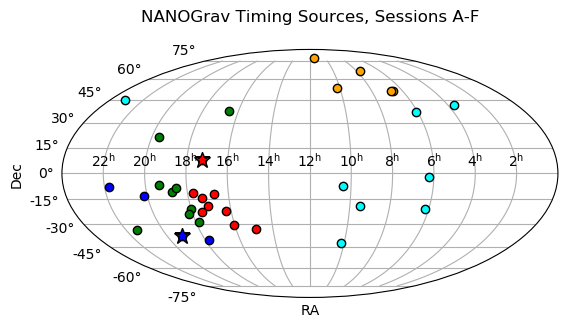
\includegraphics{nanograv_timing_sessions_12-2017.png}}
  \caption{Sky map showing distribution of timing sources: Red= A session sources, Blue= B session sources, Orange= C session sources, Cyan= D session sources, Green= E session sources, and Stars= F session sources.}
  \label{fig:map}
\end{figure}


\begin{figure}[h]
 \centering
  \scalebox{0.6}{\includegraphics{ScreenShotguppi_adc_hist.png}}
  \caption{Example of a ``good" histogram from \textbf{guppi\_adc\_hist}.  Each line comes from a different polarization, and some differences should be expected.}  
  \label{fig:gah}
\end{figure}


\begin{figure}[h]
 \centering
  \scalebox{0.5}{\includegraphics{ScreenShotScanCoord.png}}
  \caption{Scan Coordinator, showing the status of various telescope systems, including a false alarm in the IFRack status. Notice this screenshot was taken during a survey observation, so many things (e.g., receiver, project ID, source, etc.) will be different for timing observations.  }
  \label{fig:sc}
\end{figure}


\begin{figure}[h]
 \centering
  \scalebox{0.4}{\includegraphics{GUPPI_cal_screenshot.png}}
  \caption{Calibration scan example: each GPU should show the square wave ``off-on" signal, with little or no RFI.}
  \label{fig:cal}
\end{figure}


\begin{figure}[h]
 \centering
  \scalebox{0.4}{\includegraphics{GUPPI_bright_screenshot.png}}
  \caption{Bright pulsar scan example: a ``bright" pulsar in L-band should be apparent in all GPUs, in single integration (middle column) and cumulative plots (far left and right), with little or no RFI.  This pulsar could be described as ``bright, but not spectacular".  Some RFI, such as in gpu5, is normal, but shouldn't interfere significantly with pulsar signal.}
  \label{fig:bright}
\end{figure}


\begin{figure}[h]
 \centering
  \scalebox{0.4}{\includegraphics{GUPPI_faint_screenshot.png}}
  \caption{Faint pulsar scan example: a ``faint" pulsar in L-band should be apparent in the cumulative plots (far left and right) in most or all GPUs with some RFI, but may not be visible in single integrations (middle column).  This pulsar could be described as ``faint, but visible".}
  \label{fig:faint}
\end{figure}


\begin{figure}[h]
 \centering
  \scalebox{0.6}{\includegraphics{ScreenShotSkyView.png}}
  \caption{Scheduler \& SkyView, with the cursor showing the approximate position of C1045-04.  The red curve shows the galaxy, and the black curve shows the Declination of the telescope.}
  \label{fig:ssv}
\end{figure}




\end{document}  

